\documentclass[a4paper,12pt,english]{article}
\usepackage{glossaries}
\usepackage[T1]{fontenc}
\usepackage{babel}
\usepackage{graphicx}
\usepackage[table,xcdraw]{xcolor}
\usepackage{hyperref}
\usepackage{blindtext}
\usepackage{geometry}
\usepackage{parskip}
\usepackage{mathtools}
\usepackage{siunitx}
\usepackage{listings}
\usepackage{csquotes}
\usepackage{caption}
\usepackage{subcaption}
\usepackage{comment}
\usepackage{pdfpages}
\usepackage[useregional]{datetime2}
\usepackage{amsmath} % for the equation* environment
\usepackage{float}
\usepackage{pict2e}
\usepackage{fixltx2e}
\usepackage{tocloft}
\usepackage{graphicx}
\usepackage{xcolor}
\usepackage{float}
\usepackage{textgreek}
\usepackage{colortbl}

%%gmedina solution
\newcommand{\listequationsname}{List of equations}
\newlistof{myequations}{equ}{\listequationsname}
\newcommand{\myequations}[1]{%
\addcontentsline{equ}{myequations}{\protect\numberline{\theequation}#1}\par}
\setlength{\cftmyequationsnumwidth}{2.5em}% Width of equation number in List of Equations

\DeclareRobustCommand{\slashcirc}{{\mathpalette\doslashcirc\relax}}

\makeatletter
\newcommand\doslashcirc[2]{%
  \sbox\z@{$#1\m@th\circ$}%
  \setlength\unitlength{\wd\z@}
  \begin{picture}(1,1)
  \roundcap
  \put(0,0){\box\z@}
  \put(0,0){\line(1,1){1}}
  \end{picture}%
}
\makeatother


% %% Some packages you will need
% \usepackage{pgfplots}
% \usepackage{pgfplotstable}
% \usepackage{booktabs}
% \usepackage{array}



\definecolor{arduinoorange}{HTML}{FFA500}
\definecolor{arduinogray}{HTML}{808080}
\definecolor{arduinoblue}{HTML}{007ACC}
\definecolor{arduinogreen}{HTML}{469B00}

\lstset{
  language=C++,
  basicstyle=\ttfamily\footnotesize,
  keywordstyle=\color{arduinoorange},
  stringstyle=\color{arduinogreen},
  commentstyle=\color{arduinogray},
  moredelim=[s][\color{arduinoblue}]{\#}{\ },
  morekeywords={digitalRead,digitalWrite,pinMode,analogRead,analogWrite,Serial,begin,HIGH,LOW},
  frame=tb,
  tabsize=4,
  showstringspaces=false,
  breaklines=true,
  numbers=left,
  numberstyle=\tiny\color{arduinogray},
  numbersep=5pt,
  extendedchars=true,
  literate={á}{{\'a}}1 {ã}{{\~a}}1 {é}{{\'e}}1,
}

\lstdefinestyle{Arduino}
{
  language=C++,
  basicstyle=\ttfamily\footnotesize,
  keywordstyle=\color{arduinoorange},
  stringstyle=\color{arduinogreen},
  commentstyle=\color{arduinogray},
  moredelim=[s][\color{arduinoblue}]{\#}{\ },
  morekeywords={digitalRead,digitalWrite,pinMode,analogRead,analogWrite,Serial,begin},
  frame=tb,
  tabsize=4,
  showstringspaces=false,
  breaklines=true,
  numbers=left,
  numberstyle=\tiny\color{arduinogray},
  numbersep=5pt,
  extendedchars=true,
  literate={á}{{\'a}}1 {ã}{{\~a}}1 {é}{{\'e}}1,
  backgroundcolor=\color{black!85},
  rulecolor=\color{arduinoorange},
  frame=single,
  frameround=tttt,
  framexleftmargin=6pt,
  framexrightmargin=6pt,
  framextopmargin=6pt,
  framexbottommargin=6pt,
  breaklines=true,
  postbreak=\raisebox{0ex}[0ex][0ex]{\ensuremath{\color{red}\hookrightarrow\space}},
}

\usepackage[
    backend=biber,
    backref=true,
    backrefstyle=none,
    sortcites=true,
    sorting=none,
    doi=false, % doi informatie wordt niet weergegeven
    %uniquename=true,
    %uniquelist=true,
    maxcitenames=3,
    %issn=false, werkt niet
    language=american
]{biblatex}
\addbibresource{information/Sources.bib}
\DefineBibliographyStrings{english}{
    backrefpage = {blz.},
    backrefpages = {blz.},
}
\makeglossaries
\definecolor{Grey1}{HTML}{343434}
\graphicspath{{./img}}
 \geometry{
 a4paper,
 total={170mm,257mm},
 left=20mm,
 top=20mm,
 }
\hypersetup{
    colorlinks=true,
    linkcolor=blue,
    filecolor=magenta,      
    urlcolor=cyan,
    pdftitle={Overleaf Example},
    pdfpagemode=FullScreen,
    }


\begin{document}
\title{

\includegraphics[width=3.5in]{img/Logo/Logo.png} \\
\vspace*{1in}
\textbf{Project 4}\\
\textit{Plan of Approach}\\
Version 1
}
\author{
\vspace*{0.5in} \\
  Written by:\\
  Laurens van der Drift\\
  Justin van der Reijden\\
  Luuk van Kappel\\
  Marnix Harmsen\\
		\vspace*{0.2in} \\
		The Hague University of Applied Sciences\\
        \textbf{Electrical Engineering}\\
        Delft, The Netherlands
       } 
\maketitle
\phantomsection
\section*{Version History} \addcontentsline{toc}{section}{Version History}

\begin{table}[h]
\begin{tabular}{|l|l|l|l|}
\hline
\rowcolor[HTML]{4472C4} 
{\color[HTML]{FFFFFF} \textbf{Version}} &
  {\color[HTML]{FFFFFF} \textbf{Date}} &
  {\color[HTML]{FFFFFF} \textbf{Changes}} &
  {\color[HTML]{FFFFFF} \textbf{Author}} \\ \hline
\rowcolor[HTML]{D9E1F2} 
1.0 &
  \multicolumn{1}{c|}{\cellcolor[HTML]{D9E1F2}05-02-2024} &
 N.v.t. &
  Alset Innovations \\ \hline

% \rowcolor[HTML]{FFFFFF} 
% 2.0 &
%   \multicolumn{1}{c|}{\cellcolor[HTML]{FFFFFF}7-4-2023} &
%  Feedback van FeedbackFruits toegepast &
%   Infra   Vroom \\ \hline

% \rowcolor[HTML]{D9E1F2} 
% 3.0 &
%   \multicolumn{1}{c|}{\cellcolor[HTML]{D9E1F2}4-6-2023} &
%  Bijgewerkt voor Assessment 3 &
%   Infra   Vroom \\ \hline

\end{tabular}
\end{table}
%\addcontentsline{toc}{section}{Verklarende Woordenlijst}
\printglossaries
\newglossaryentry{tender}
{
    name=\textit{tender},
    description={De inschrijving om op een kavel een wind turbine park te bouwen.}
}

\phantomsection
\addcontentsline{toc}{section}{List of Figures}
\listoffigures

\newpage
\tableofcontents
\section{STM32F411CEU6}
\subsection{Why this MCU?}
Our choice of the STM32F411CEU6 stems from a commitment to innovation, steering away from the common trend of utilizing a Pi Zero, a path often trodden by other groups. Delving into the intricacies of our decision, let's explore the schematic in \autoref{fig:Blackpill_STM32F411CEU6_Schematic}.
\begin{figure}[H]
    \centering
    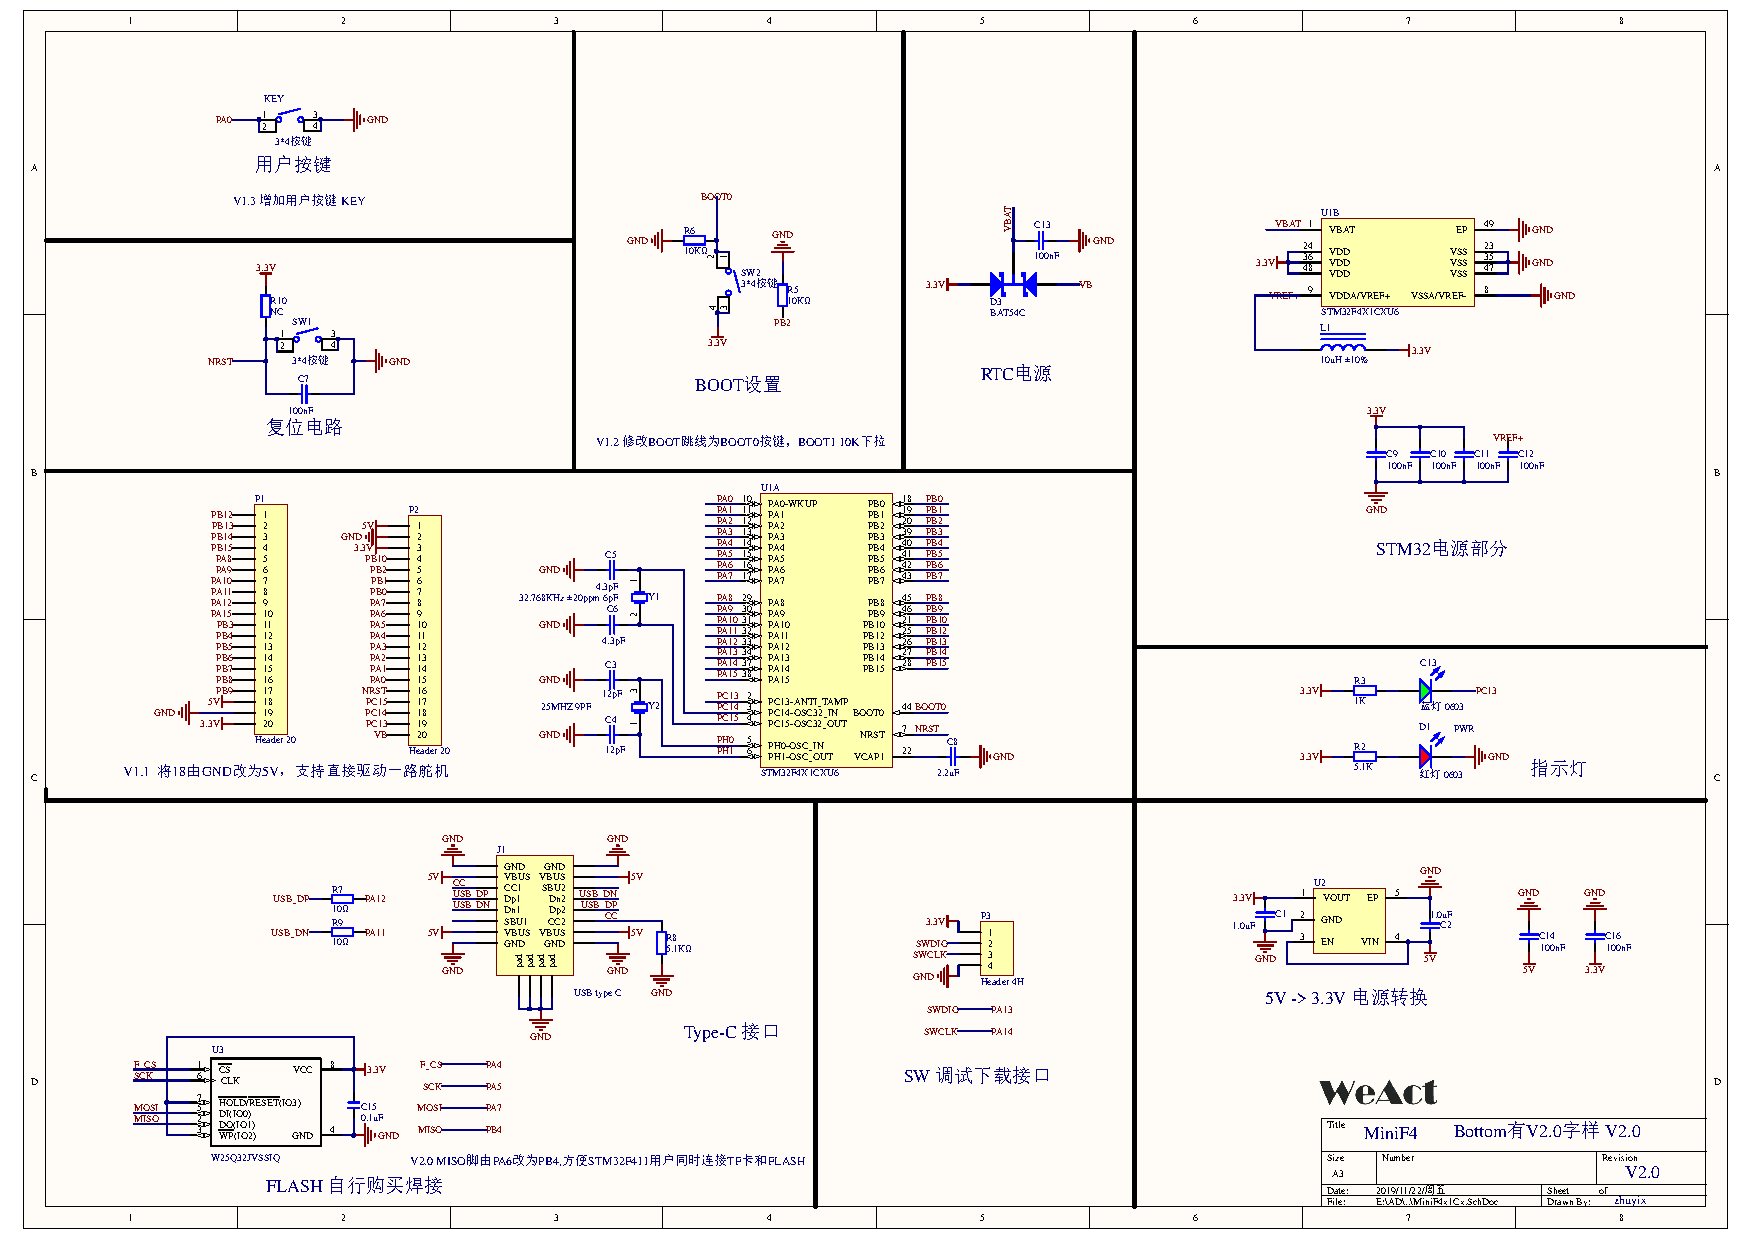
\includegraphics[width=1\linewidth]{img//blackpill/original-schematic-STM32F411CEU6_WeAct_Black_Pill_V2.0.pdf}
    \caption{Blackpill STM32F411CEU6 Schematic}
    \label{fig:Blackpill_STM32F411CEU6_Schematic}
\end{figure}
\begin{itemize}
    \item \textbf{Circuit with Buttons:} The schematic reveals a carefully designed circuit accommodating essential buttons - Key, Switch, and Boot - crucial for operational control.

    \item \textbf{Real-Time Clock (RTC):} A dedicated circuit for real-time clock functionality ensures precise timing and synchronization within our motor control system.

    \item \textbf{STM32F411CEU6 Pinout:} The MCU itself is dissected with a pinout, providing insights into the connections and functionalities of each pin.

    \item \textbf{Flash Circuit:} A specialized flash circuit, integral for storing and retrieving data, contributes to the robust performance of our system.

    \item \textbf{Voltage Regulator:} The presence of a voltage regulator ensures stable and reliable power distribution throughout the system.

    \item \textbf{Additional Circuits:} Beyond these components, the schematic highlights several other circuits vital for the holistic functionality of our design.
\end{itemize}

Moving from the abstract schematic to the tangible layout, the dimensions in \autoref{fig:Blackpill_STM32F411CEU6_Dimensions} depict the spatial arrangement of each component. Assembled into a cohesive unit, the complete PCB with the integrated STM32F411CEU6 is visualized in \autoref{fig:Blackpill_STM32F411CEU6_Picture}.
\begin{figure}[H]
    \centering
    \begin{subfigure}{0.48\textwidth}
        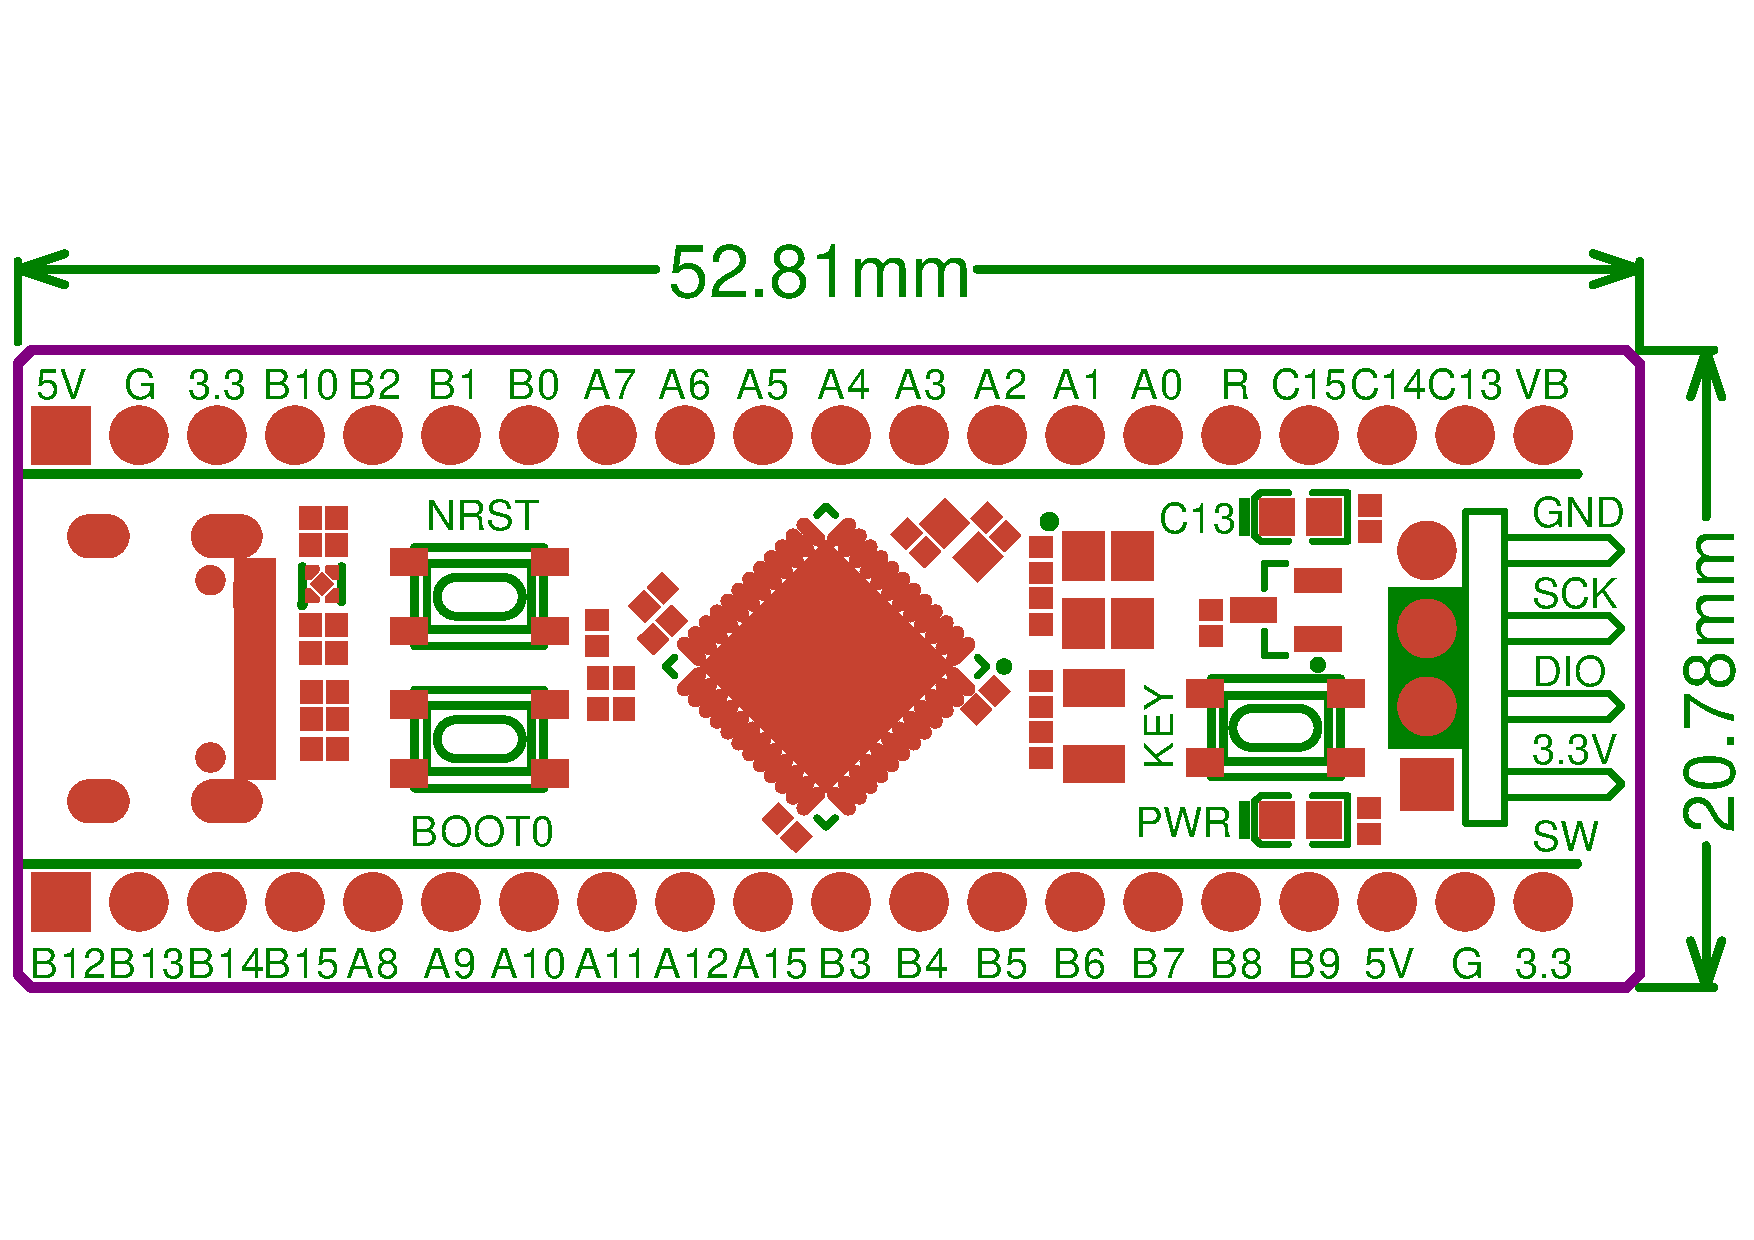
\includegraphics[width=\linewidth]{img/blackpill/original-dimensions-STM32F411CEU6_WeAct_Black_Pill_V2.0.pdf}
        \caption{Blackpill STM32F411CEU6 Dimensions}
        \label{fig:Blackpill_STM32F411CEU6_Dimensions}
    \end{subfigure}
    \hfill
    \begin{subfigure}{0.48\textwidth}
        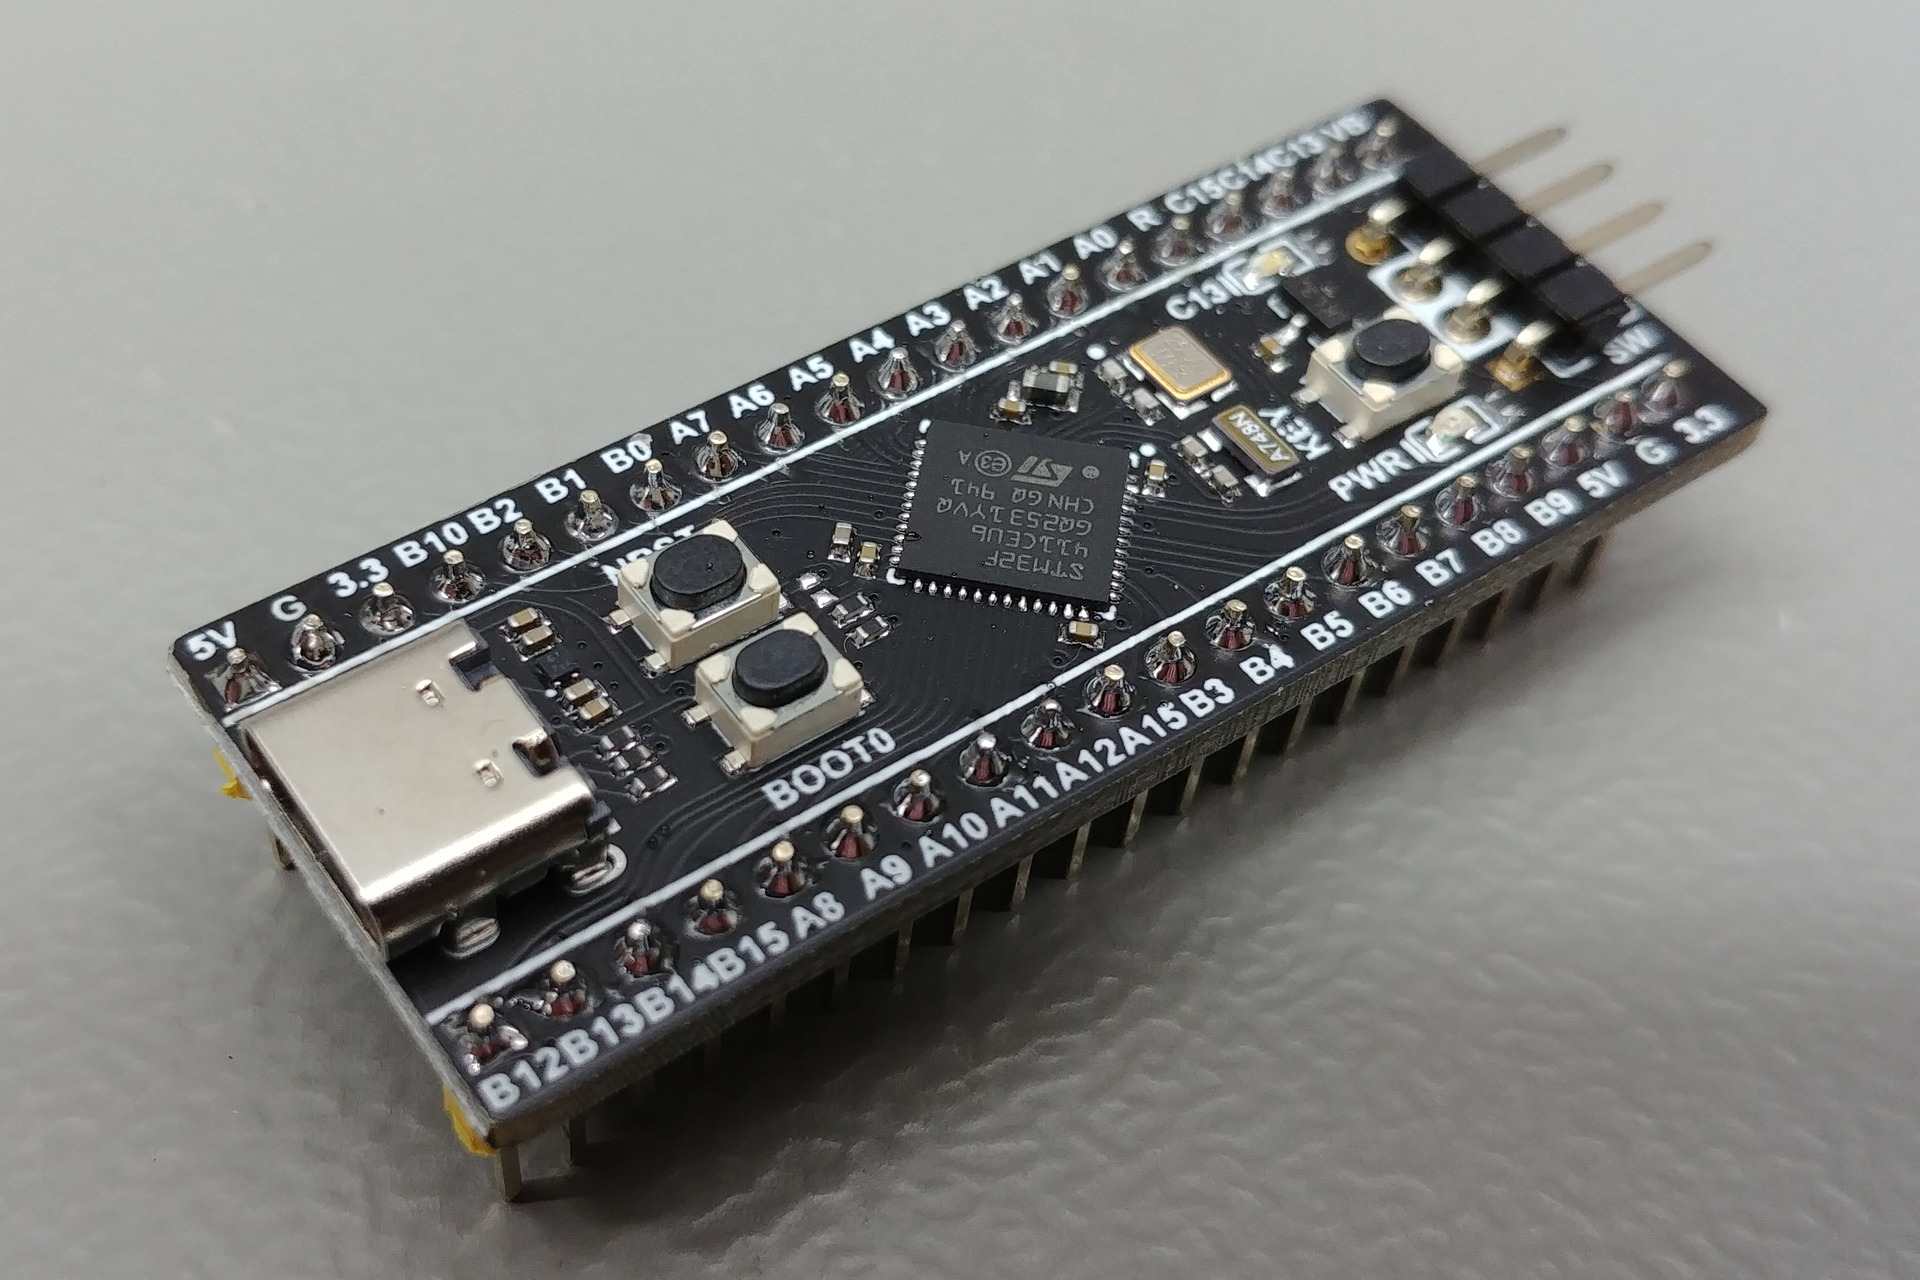
\includegraphics[width=\linewidth]{img/blackpill/STM32F411CEU6_WeAct_Black_Pill_V2.0-1.jpg}
    \caption{Blackpill STM32F411CEU6 Picture}
    \label{fig:Blackpill_STM32F411CEU6_Picture}
    \end{subfigure}
\end{figure}

\subsection{Specifications}
    \subsubsection{Microcontroller:}
    \begin{itemize}
        \item Part: STM32F411CEU6
        \item Manufacturer: ST-Microelectronics
        \item Core: Arm Cortex-M4
        \item Max. Clock Speed: 100MHz
        \item Package: UFQFPN 48 pins
    \end{itemize}

    \subsubsection{Internal Memories:}
    \begin{itemize}
        \item FLASH: 512KiB
        \item SRAM: 128KiB
    \end{itemize}

    \subsubsection{Oscillators:}
    \begin{itemize}
        \item HSI: 16MHz
        \item HSE: 25MHz (Critical for precise motor control)
        \item LSI: 32kHz
        \item LSE: 32.768kHz
    \end{itemize}

    \subsubsection{Power:}
    \begin{itemize}
        \item Voltage Input: +3.52V to +5.25V
        \item Power Sources: Any +3.3V pin, Any +5V pin, USB connector
        \item Backup battery: Supported
    \end{itemize}

    \subsubsection{Regulator:}
    \begin{itemize}
        \item Manufacturer: Diodes Incorporated
        \item Part: AP7343 (6T)
        \item Input: +3.52V to +5.25V
        \item Output: +3.3V @ 300mA
    \end{itemize}

    \subsubsection{PCB:}
    \begin{itemize}
        \item Color: Black
        \item Size (w x l): 20.78mm x 52.81mm
        \item Mounting: Breadboard
    \end{itemize}

    \subsubsection{Inputs \& Outputs:}
    \begin{itemize}
        \item Reset button (Active low)
        \item BOOT0 button (Active high)
        \item User button (Active low)
        \item Power LED (Connected to +3.3V rail)
        \item User LED (Connected to PC13)
    \end{itemize}

    \subsubsection{Connectors \& Headers:}
    \begin{itemize}
        \item Header 1 (20x1, male): 5V, GND, 3.3V, Motor Control Pins (PB0-PB10, PA0-PA7, PC13, NRST, PC15, PC14, VBAT)
        \item Header 2 (20x1, male): Motor Control Pins (PB12-PB15, PA8-PA15, PB3-PB9, 5V, GND, 3.3V)
        \item USB Connector (USB C): VBUS, D-, D+, GND (For potential external communication)
        \item SWD Header (4x1, male): 3.3V, SWDIO (PA13), SWCLK (PA14), GND (For debugging and programming)
    \end{itemize}

    \subsubsection{Devices:}
    \begin{itemize}
        \item Generic EEPROM (I2C): SOP 8 pins, Generic I2C EEPROM
        \item Connected to PA4 (CS), PB4 (DO), +3.3V rail (WP, HOLD), Ground plane (GND), PA7 (DI), PA5 (CLK), +3.3V rail (VCC)
    \end{itemize}

All information from this section has been retrieved thru these sources \cite{stm32datasheet,stm32base,stmicro}.
\section{Hall sensor}
\subsection{What is a hall sensor?}
A Hall sensor is a transducer that varies its output voltage in response to changes in the magnetic field. It is often used to detect the presence or absence of a magnetic field and to measure the strength and polarity of the field. The Hall sensor operates on the principle of the Hall effect, where a voltage difference is created across a conductor when it is subjected to a magnetic field perpendicular to the current flow.\cite{9568879}

\subsection{What does a hall sensor do in our application?}
In our application, the Hall sensors play a crucial role in providing feedback on the rotor position of the Brushless Direct Current (BLDC) motor. The three Hall sensors are strategically placed around the motor to detect the magnetic field generated by the rotating magnets in the rotor. By monitoring the Hall sensor outputs, we can determine the rotor's position, allowing precise control of the motor and enabling closed-loop operation.\cite{7489411}

\subsection{Hardware}
For the hardware setup, initial attempts to read out values on the oscilloscope were unsuccessful. After consulting with Diego Zuidervliet\cite{zuidervliet2024}, it was suggested to add either a pull-up or pull-down resistor to stabilize the Hall sensor outputs.

A pull-up resistor connects the sensor output to a high voltage level, and a pull-down resistor connects it to a low voltage level. The purpose is to ensure a defined voltage level when the sensor is not actively providing a signal. In our case, we added a 10K ohm pull-up resistor to each Hall sensor output.

The wiring diagram, shown in \autoref{fig:hall_sensor_wiring_diagram}, depicts the connection of the pull-up resistors to the Hall sensor outputs. With this modification, we successfully plotted the Hall sensor information on the oscilloscope, providing stable and readable output.

\begin{figure}[H]
    \centering
    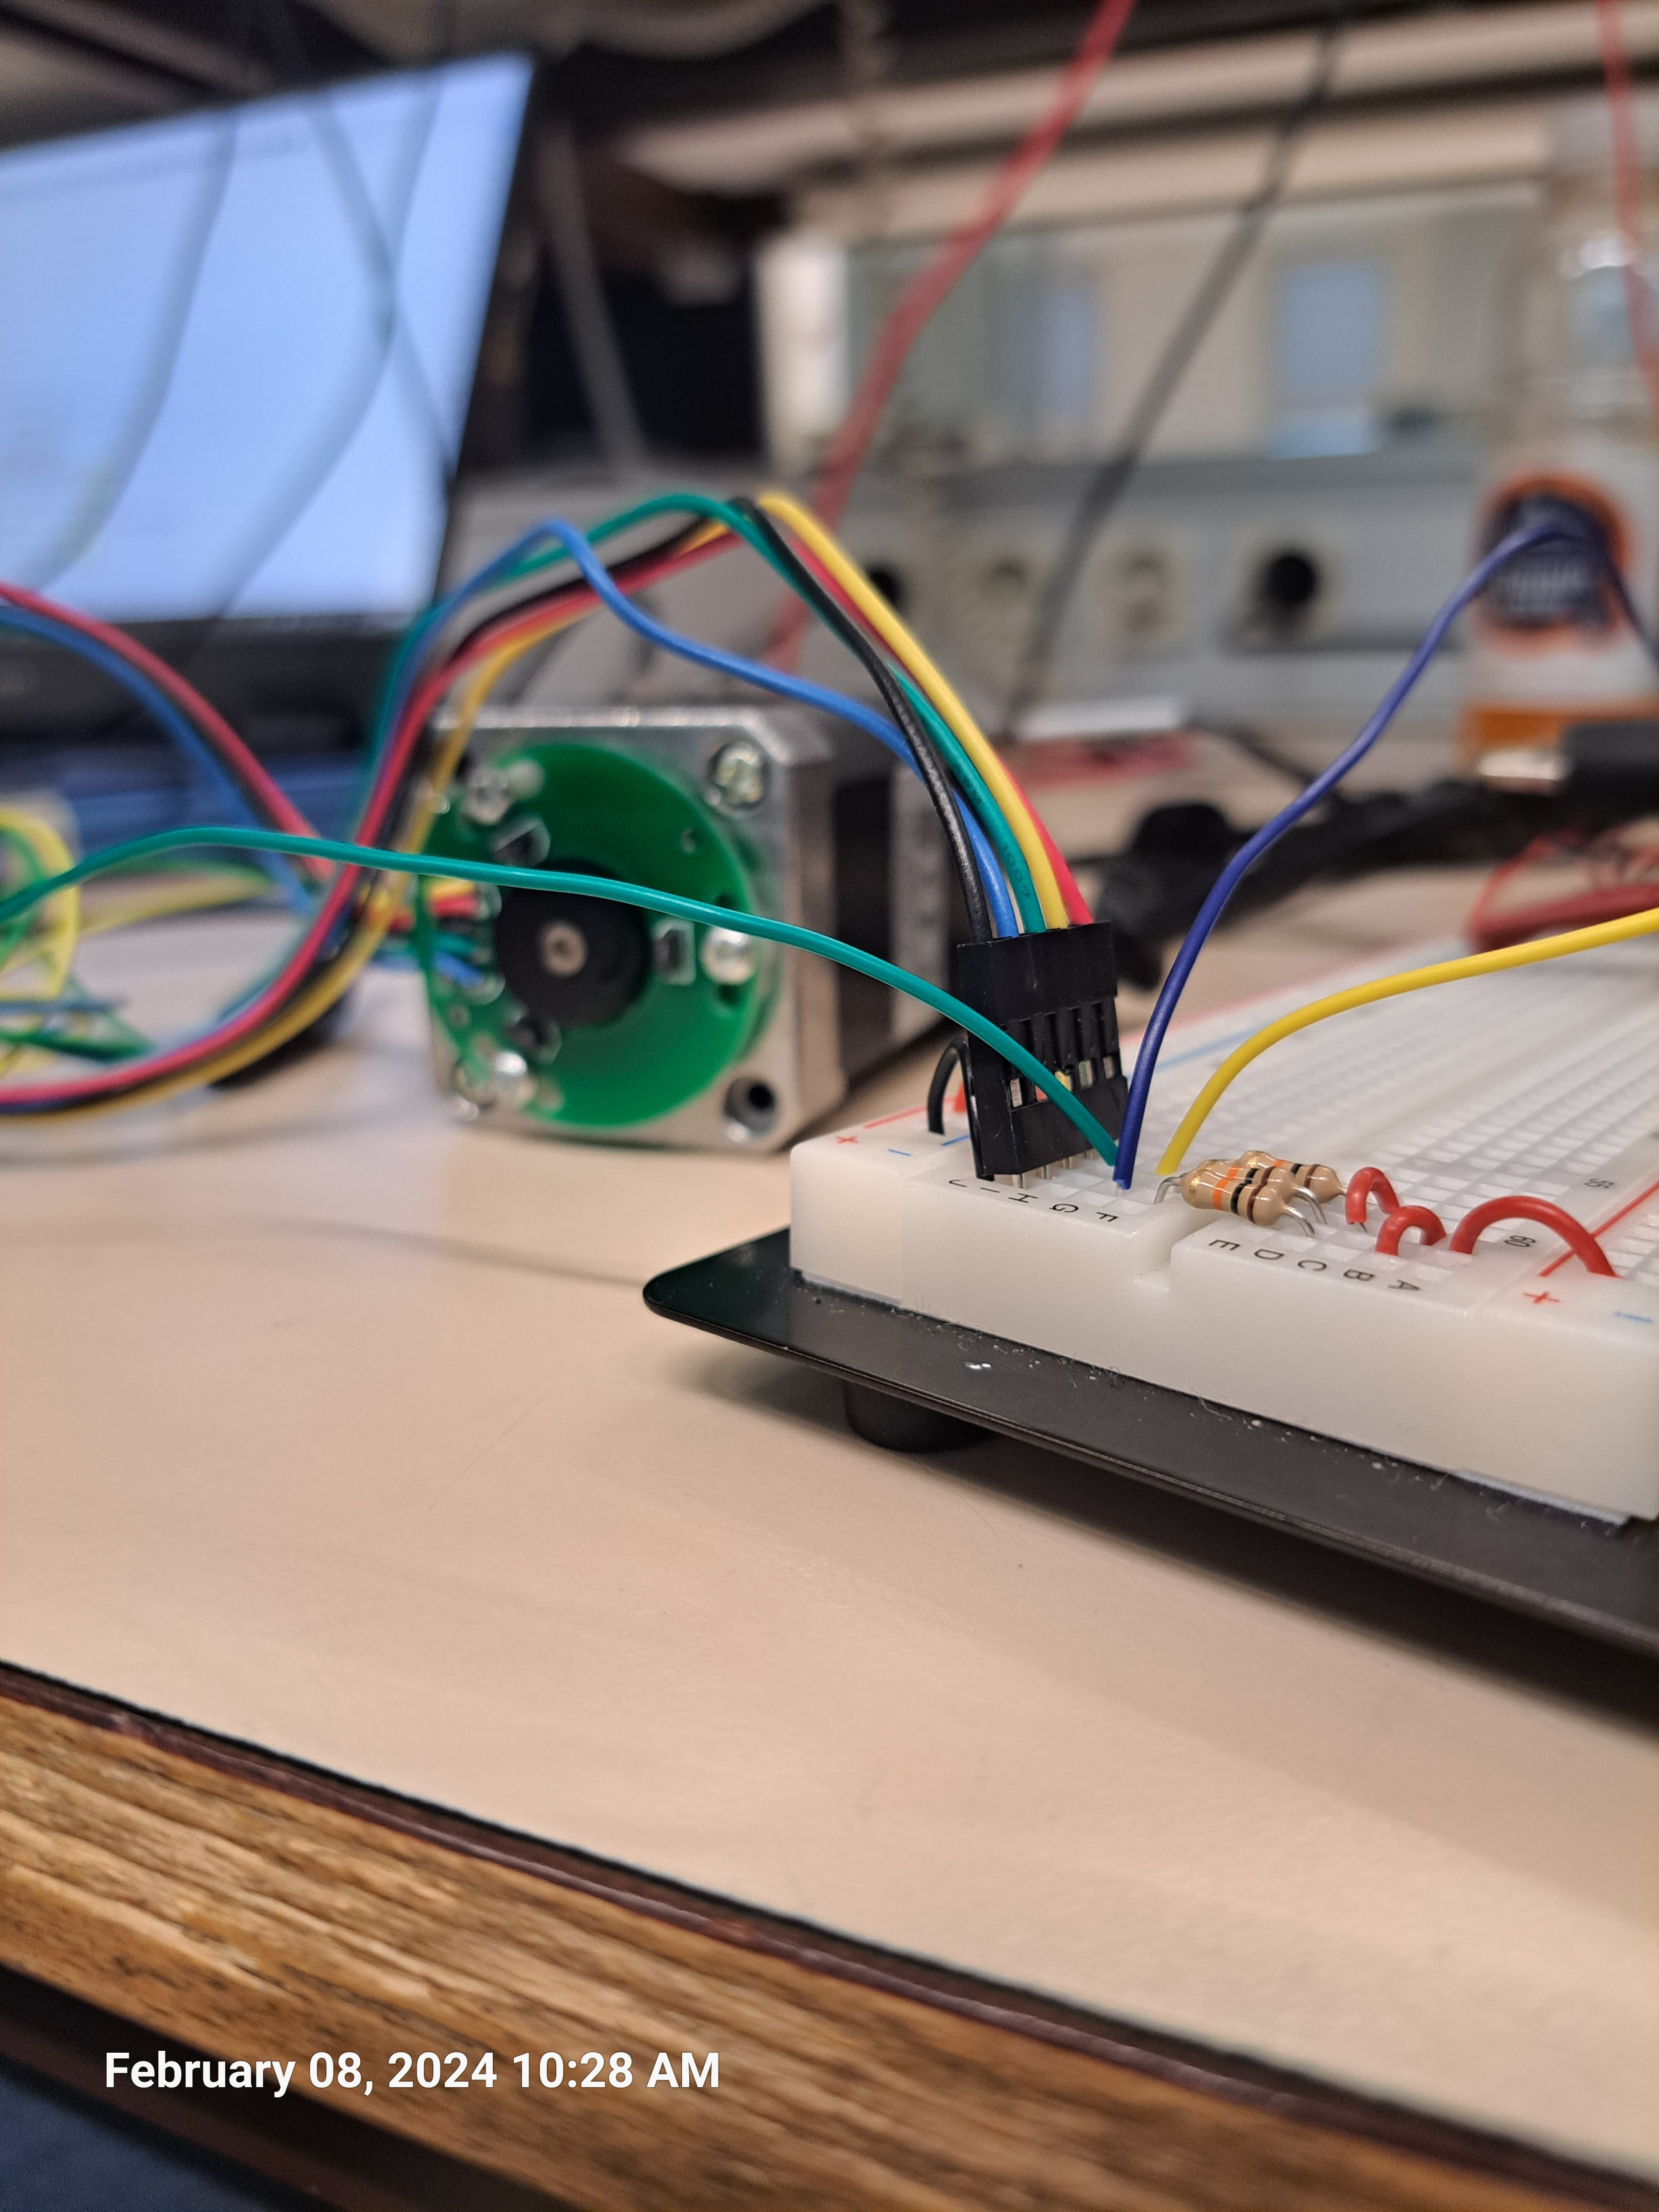
\includegraphics[width=0.3\textwidth]{img/Testing_Hallsensor_8-2-2024/Pictures/pull-up-resistor-breadboard-and-hall-sensor2.jpg}
    \caption{Wiring Diagram with Pull-up Resistors}
    \label{fig:hall_sensor_wiring_diagram}
\end{figure}

The circuit diagram, shown in \autoref{fig:hall_sensor_circuit_diagram}, illustrates the connection of the Hall sensors with the pull-up resistors.

\begin{figure}[H]
    \centering
    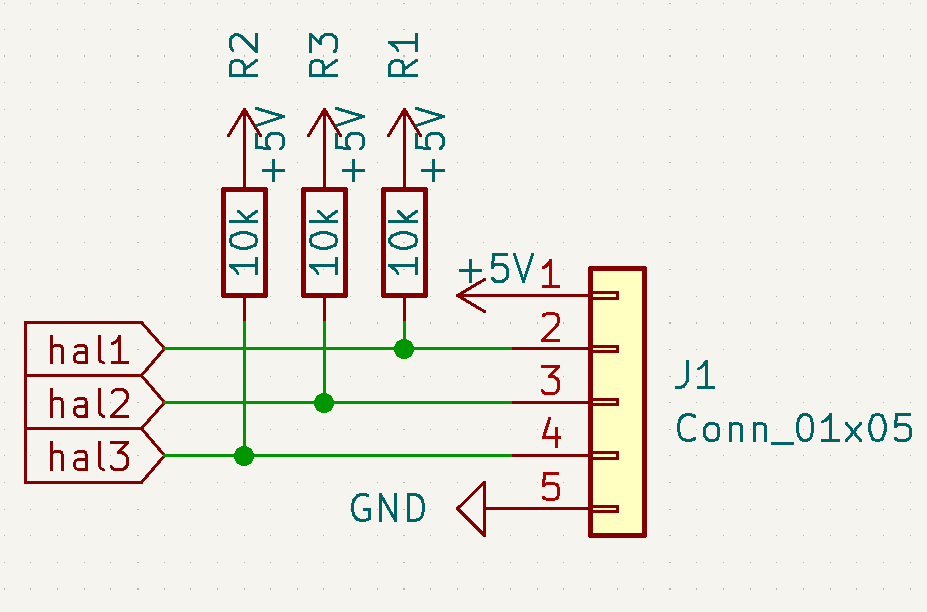
\includegraphics[width=0.45\textwidth]{img/Testing_Hallsensor_8-2-2024/Circuit/hall_sensor_circuit.png}
    \caption{Circuit Diagram with Pull-up Resistors}
    \label{fig:hall_sensor_circuit_diagram}
\end{figure}

Since we now understand the Hall sensor's function, its role in our application, and how to obtain stable readings, we can proceed with the software development.



\subsection{Software}





\phantomsection
\addcontentsline{toc}{section}{Referenties}
\printbibliography
\end{document}
